\documentclass[11pt,a4paper]{article}
\usepackage[margin=23mm]{geometry}
\usepackage[T1]{fontenc}
\usepackage{lmodern,microtype}
\usepackage{amsmath,amssymb,booktabs,graphicx}
\usepackage{parskip,enumitem}
\usepackage[hidelinks]{hyperref}
\usepackage{caption,float}
\captionsetup{font=small,labelfont=bf}
\setlength{\emergencystretch}{3em}
\setlist{itemsep=2pt,topsep=4pt}
\title{Paper revisions for supervisor review}
\author{Replacement passages and verified recall results}
\date{9 September 2026}
\begin{document}
\maketitle
\noindent\textbf{Scope.} This pack provides replacement passages for the
supplied manuscript. The primary cultural result and original model-level
recall intervals are preserved. Newly calculated comparisons are labelled
exploratory. The original PDF has not been altered.

\noindent\textbf{Main change.} Explain matching decisions before recall,
then present RQ1 (WEIRD--Serbian), RQ2 (model performance), RQ3
(US--China), and descriptive judge checks in that order. The accompanying
\texttt{revision\_notes.md} explains every change and gives reproducibility
details. \texttt{replacement\_sections.tex} contains the editable passages.

\noindent\textbf{Category correction.} The table separates five
Frontier/API systems, six larger open-weight systems, and two smaller
open-weight systems. Qwen 3.7 Max moves from the original mixed middle
tier to the API group: official documentation describes a commercial
API flagship, and a public-weight release was not verified. The categories
describe access and relative size, not a capability ranking. Original-tier
summaries remain in the analysis files for comparison; no model is dropped.

\noindent\textbf{Integration.} Copy the indicated passages into the current
source, update cross-references and the model-category definition, and move
the original precision/F1 table into the supplementary material. The
unaffected introduction, related work, topic construction, prompts,
bibliography and other original material remain in the submission source.

\clearpage
% Replacement passages for the supplied manuscript. Copy the relevant blocks.
% Requires amsmath, amssymb, booktabs, graphicx, float. The wrapper supplies these.
% Preserve the manuscript's other sections, bibliography and archived prompts.

\section*{Abstract: replacement result sentences}
Mean recall was 0.581 for WEIRD topics and 0.594 for Serbian topics.
Across the eight matched topic pairs, the mean WEIRD-minus-Serbian difference
was $-0.013$, or $-1.3$ percentage points (95\% bootstrap CI: $-8.1$ to
$5.8$ percentage points). An exact one-sided Wilcoxon signed-rank test on
the eight pair-level differences provided no evidence for the hypothesised
WEIRD recall advantage ($p=0.680$).

\section*{Introduction: replacement research questions}
We address three research questions:
\begin{description}
\item[RQ1 (primary).] Do LLMs recover fewer documented perspectives on
Serbian sociopolitical topics than on structurally matched WEIRD topics?
We hypothesise higher recall on the WEIRD topics.
\item[RQ2 (exploratory).] How does perspective recall vary across individual
models, frontier API systems, and larger and smaller open-weight systems?
\item[RQ3 (exploratory).] How do the selected models from US and Chinese
developers differ in overall recall and in their WEIRD--Serbian recall gaps?
\end{description}
Recall is the principal outcome for all three questions because the study
concerns recovery of a fixed set of documented perspectives. Precision and
F1 are supplementary descriptions of matching behaviour. The additional
category and developer-country comparisons are exploratory.

\setcounter{section}{2}
\section{Methodology: replacement subsections}
\setcounter{subsection}{2}
\subsection{Judge evaluation}
\label{sec:judge-evaluation}
The judges make matching decisions; recall is calculated after these
decisions have been collected. For each model and topic, the model produces
five perspectives. Each of five LLM judges receives one generated
perspective at a time, together with the topic's five reference perspectives.
The judge selects the reference that expresses the same underlying stance,
or returns \emph{no match}. This produces five decisions per generated
perspective and 25 decisions per model--topic response when all calls succeed.
Judges do not receive one another's decisions.

We use \emph{family-disjoint judging}: no judge belongs to the same
developer family as the generator whose output it evaluates. Here, a family
is the developer grouping used in the evaluation configuration. For example,
Gemini and Gemma belong to the Google family, GPT and GPT-OSS to OpenAI,
and Claude Opus and Claude Sonnet to Anthropic. The five judges in each
realised panel also come from distinct developer families.

The base panel consists of Gemini 3.1 Pro (Google), GPT 5.5 (OpenAI),
Claude Sonnet 5 (Anthropic), DeepSeek V4 Pro (DeepSeek), and Kimi K2.6
(Moonshot). If the generator shares a family with a base-panel judge, we
replace that judge with a designated substitute. Grok 4.5 replaces the
Google, OpenAI, Anthropic, or Moonshot judge when necessary; Qwen 3.7 Max
replaces the DeepSeek judge. Other generators use the unchanged base panel.
This procedure prevents same-family evaluation, but does not establish
that the judges are free from shared biases.

The reference order is randomised independently for every judgment.
Returned indices are mapped back to the original reference identifiers
before scores are calculated. Of 5,200 intended decisions, 5,184 are valid
after retries. There are 1,024 generated perspectives with five valid
judgments and 16 with four. A failed call is treated as missing data;
a valid no-match decision is retained and contributes zero credit.

\subsection{Calculating perspective recall}
\label{sec:recall}
Recall measures the proportion of the five reference perspectives recovered
in a model's five outputs. We use it as the primary metric because the
evaluation target is a finite set of documented positions, and RQ1 concerns
which of those positions are omitted. The five-output budget gives every
model the same opportunity to recover that set. Repeating a position uses
an output slot without covering an additional reference.

\paragraph{Step 1: interpret one judge's assignments.}
Suppose a judge assigns the five generated perspectives to
\[
1,\quad 2,\quad 2,\quad 4,\quad \text{no match}.
\]
Three distinct references have been recovered: 1, 2, and 4. This judge's
recall for the model--topic response is therefore
\[
R_j = \frac{\text{number of distinct references recovered}}{5}
    = \frac{3}{5}=0.60.
\]
The repeated match to reference 2 does not increase recall. Although four
outputs match a reference, they cover only three distinct positions.

\paragraph{Step 2: combine the judges' assessments.}
When all five judges evaluate all five outputs, topic recall equals the
mean of their five distinct-reference recalls:
\[
R_{mt}=\frac{1}{5}\sum_{j=1}^{5}R_{mtj}.
\]
For example, judge recalls of $0.60$, $0.60$, $0.80$, $0.40$, and $0.40$
give topic recall $0.56$. This corresponds to an average of 2.8 of the
five references recovered across judges. It does not require the judges
to agree on a single set of recovered references, and it does not apply
a majority-vote threshold.

\paragraph{Exact aggregation, including missing judgments.}
The implementation combines fractional reference credits and accounts for
missing judgments separately for each output. For a fixed model and topic,
let $y_{jk}$ be judge $j$'s assignment for generated perspective $k$,
where references are indexed by $g\in\{1,\ldots,5\}$ and zero denotes
no match. Let $n_{jg}$ be the number of available assignments by judge $j$
to reference $g$. Each assignment receives credit
\begin{equation}
c_{jkg}=\begin{cases}
1/n_{jg}, & y_{jk}=g,\\
0, & \text{otherwise}.
\end{cases}
\label{eq:split-credit}
\end{equation}
Thus, two matches to the same reference receive one half each; together
they contribute one unit for that judge. If $J_k$ contains the judges
with a valid decision for output $k$, the panel credit is
\begin{equation}
w_{kg}=\frac{1}{|J_k|}\sum_{j\in J_k}c_{jkg}.
\label{eq:panel-credit}
\end{equation}
We sum these credits for each reference, cap the sum at one, and average
across the five references:
\begin{equation}
C_g=\min\!\left(1,\sum_{k=1}^{5}w_{kg}\right),
\qquad
R_{mt}=\frac{1}{5}\sum_{g=1}^{5}C_g.
\label{eq:topic-recall}
\end{equation}
With complete panels, these equations reduce to the mean judge recall
given above. When judgments are missing, $|J_k|$ can differ across outputs;
the cap prevents any reference receiving more than full credit. All outputs
in this dataset have at least four valid judgments.

\paragraph{Step 3: summarise topics and models.}
Each topic receives equal weight. Overall model recall is the mean of
the 16 topic recalls. WEIRD recall and Serbian recall are the corresponding
means over eight topics each. Therefore,
\begin{equation}
\overline R_m=\frac{1}{16}\sum_{t=1}^{16}R_{mt}
=\frac{\overline R_m^{\mathrm W}+\overline R_m^{\mathrm S}}{2}.
\label{eq:model-recall}
\end{equation}
Recall describes coverage of the benchmark's reference set. It does not
measure coverage of every legitimate position that may exist outside it.

\subsection{Statistical analysis}
\label{sec:statistics}
\paragraph{RQ1: the primary matched-topic comparison.}
For each generator $m\in\{1,\ldots,13\}$ and matched topic pair
$p\in\{1,\ldots,8\}$, we calculate
\begin{equation}
d_{mp}=R_{mp}^{\mathrm W}-R_{mp}^{\mathrm S}.
\end{equation}
Positive differences favour WEIRD topics. The resulting $13\times8$
matrix contains 104 paired differences. We average across generators
within each pair,
\begin{equation}
\Delta_p=\frac{1}{13}\sum_{m=1}^{13}d_{mp},
\end{equation}
and apply an exact one-sided Wilcoxon signed-rank test to the eight
$\Delta_p$ values. The directional alternative is a positive shift,
corresponding to the predicted WEIRD advantage. We also report the two-sided
test. The signed-rank inference assumes independent pair-level differences
with a symmetric distribution under the null; it is not a direct test of
the arithmetic mean. The mean difference and its 95\% percentile bootstrap
interval summarise effect size. The interval uses 10,000 resamples of the
eight matched pairs, keeping all 13 models together within each sampled pair.

\paragraph{RQ1: exploratory sensitivity analyses.}
We examine the alternative aggregation across pairs within each model,
$\overline d_m=\frac18\sum_p d_{mp}$, and apply an exact signed-rank
calculation to these 13 model means. We remove numerical roundoff before
ranking, use average ranks for ties, and enumerate every sign assignment.
This comparison is conditional on the same eight topic pairs and does
not make the selected model families independent cultural replications.

To examine variation across both dimensions, we also resample generator
rows and matched-pair columns independently with replacement, retaining
the Cartesian-product submatrix in each of 10,000 replicates. This crossed
bootstrap provides an approximate interval for the mean gap.\footnote{The
resampling scheme follows Owen (2007), \emph{The pigeonhole bootstrap},
\href{https://arxiv.org/abs/0712.1111}{arXiv:0712.1111}.}
A supplementary
crossed random-intercept model provides a separate model-based check:
\begin{equation}
d_{mp}=\mu+u_m+v_p+\epsilon_{mp},
\label{eq:crossed}
\end{equation}
with independent random intercepts for generator and matched pair and
an independent residual. We estimate it by restricted maximum likelihood
and report an approximate two-sided Wald test for $\mu$. These analyses
account for the two grouping dimensions under their respective assumptions;
they do not establish representativeness of the selected models and topics
or explicitly model dependence between different generators from one family.
We do not treat the 104 differences as independent observations.

\paragraph{RQ2: model performance.}
The main table reports overall recall and recall separately for WEIRD and
Serbian topics. We distinguish five Frontier/API systems without a verified
public-weight release for the evaluated model, six larger open-weight
systems, and two smaller open-weight systems. Qwen 3.7 Max is included
in the API group, following its documentation as a commercial API flagship,\footnote{See
\href{https://www.alibabacloud.com/en/news/product/maxcompute-model-computing-service-supports-qwen37-max-and-other-commercial-models-mkv}{Alibaba Cloud's Qwen3.7-Max commercial-model announcement}.
Public-weight release sources for the eight open-weight generators are
listed in the accompanying revision notes.}
rather than in the original mixed Strong/open-weight tier. The smaller
open-weight group contains Gemma 4 31B and Llama 3.3 70B; the remaining
six public-weight systems form the larger open-weight group. These are
operational access and relative-size categories, not a capability ranking.
All generators were evaluated through the same API-based workflow, whether
or not their weights are public. Weight availability describes the model
release, not how its outputs were generated in this experiment.
Models are ordered by recall within each category. Overall recall intervals
retain the original 10,000-resample percentile bootstrap over 16 topics.

For an exploratory comparison of category means, we first average
the two cultural-arm recalls within each model and matched pair. We then
average across models in each category, with equal model weights. Differences
between categories are tested using all $2^8=256$ sign assignments over the
eight pair-level differences. These two-sided tests assume independent,
sign-exchangeable pair-level contrasts and hold the selected models fixed.
We apply Holm correction across four overall-recall comparisons: the three
pairwise category contrasts and the API group versus all eight open-weight
models combined. The original benchmark-tier summaries are retained in
the accompanying analysis files for traceability.

\paragraph{RQ3: developer-country comparisons.}
We compare eight models from US developers with four models from Chinese
developers. Mistral, from France, is excluded from this contrast but retained
in the other analyses. The US group consists of Claude Opus 4.8, GPT 5.5,
Gemini 3.1 Pro, Grok 4.3, Llama 4 Maverick, GPT-OSS 120B, Gemma 4 31B,
and Llama 3.3 70B. The Chinese group consists of DeepSeek V4 Pro,
Qwen 3.7 Max, Kimi K2.6, and GLM 5.2.

We examine two outcomes: the difference in overall recall and the
difference in WEIRD--Serbian recall gaps. For each outcome, models receive
equal weight within their developer group, and the eight matched topic
pairs are the blocks for exact two-sided sign-flip tests. We report
10,000-resample pair-bootstrap intervals and apply Holm correction across
these two RQ3 tests. These exploratory comparisons describe the selected
systems; they do not identify a causal effect of developer country.

\paragraph{Descriptive checks on the judging procedure.}
We report Fleiss' $\kappa$, Gwet's AC1, and Krippendorff's $\alpha$
overall and by cultural arm, together with judge-level no-match rates.
Leave-one-judge-out analyses describe sensitivity to the panel's composition.
These checks assess consistency and sensitivity, not whether the matching
decisions are correct or free from shared bias.

\section{Results}
\subsection{RQ1: Recall on matched WEIRD and Serbian topics}
\label{sec:rq1}
Mean recall is 0.581 for WEIRD topics and 0.594 for Serbian topics.
Across the eight matched topic pairs, the mean WEIRD-minus-Serbian
difference is $-0.013$, or $-1.3$ percentage points (95\% bootstrap CI:
$-8.1$ to $5.8$ percentage points). The median pair-level difference
is $-0.014$.

The exact one-sided Wilcoxon signed-rank test provides no evidence for
the hypothesised WEIRD advantage ($p=0.680$). The two-sided test gives
$p=0.742$, with a matched-pairs rank-biserial correlation of $-0.17$.
The point estimate favours Serbian topics slightly, but the interval
includes differences in both directions. This result does not establish
equivalent coverage across the two settings.

Four matched pairs favour WEIRD topics and four favour Serbian topics.
The largest differences point in opposite directions: recall is 19.1
percentage points higher for German immigration than for its Serbian
migration-route counterpart, but 16.9 points lower for Canadian residential
schools than for Srebrenica. Mean topic recall ranges from 0.449 for the
Serbian migration-route topic to 0.685 for Serbia's West-versus-Russia
alignment. Both extremes occur among the Serbian topics, indicating that
topic-level variation does not follow a uniform cultural direction.

The additional sensitivity analyses lead to the same substantive
interpretation. Averaging over pairs within each model gives one-sided
$p=0.843$ and two-sided $p=0.331$. Independently resampling models and
topic pairs gives a crossed-bootstrap interval of $[-0.090,0.070]$.
The model-based crossed-effects check estimates the same mean gap,
$-0.013$ (SE $0.038$; 95\% Wald CI $[-0.088,0.062]$; two-sided
$p=0.733$). These are supplementary checks; the eight-pair test remains
the primary analysis.

\begin{figure}[H]
\centering
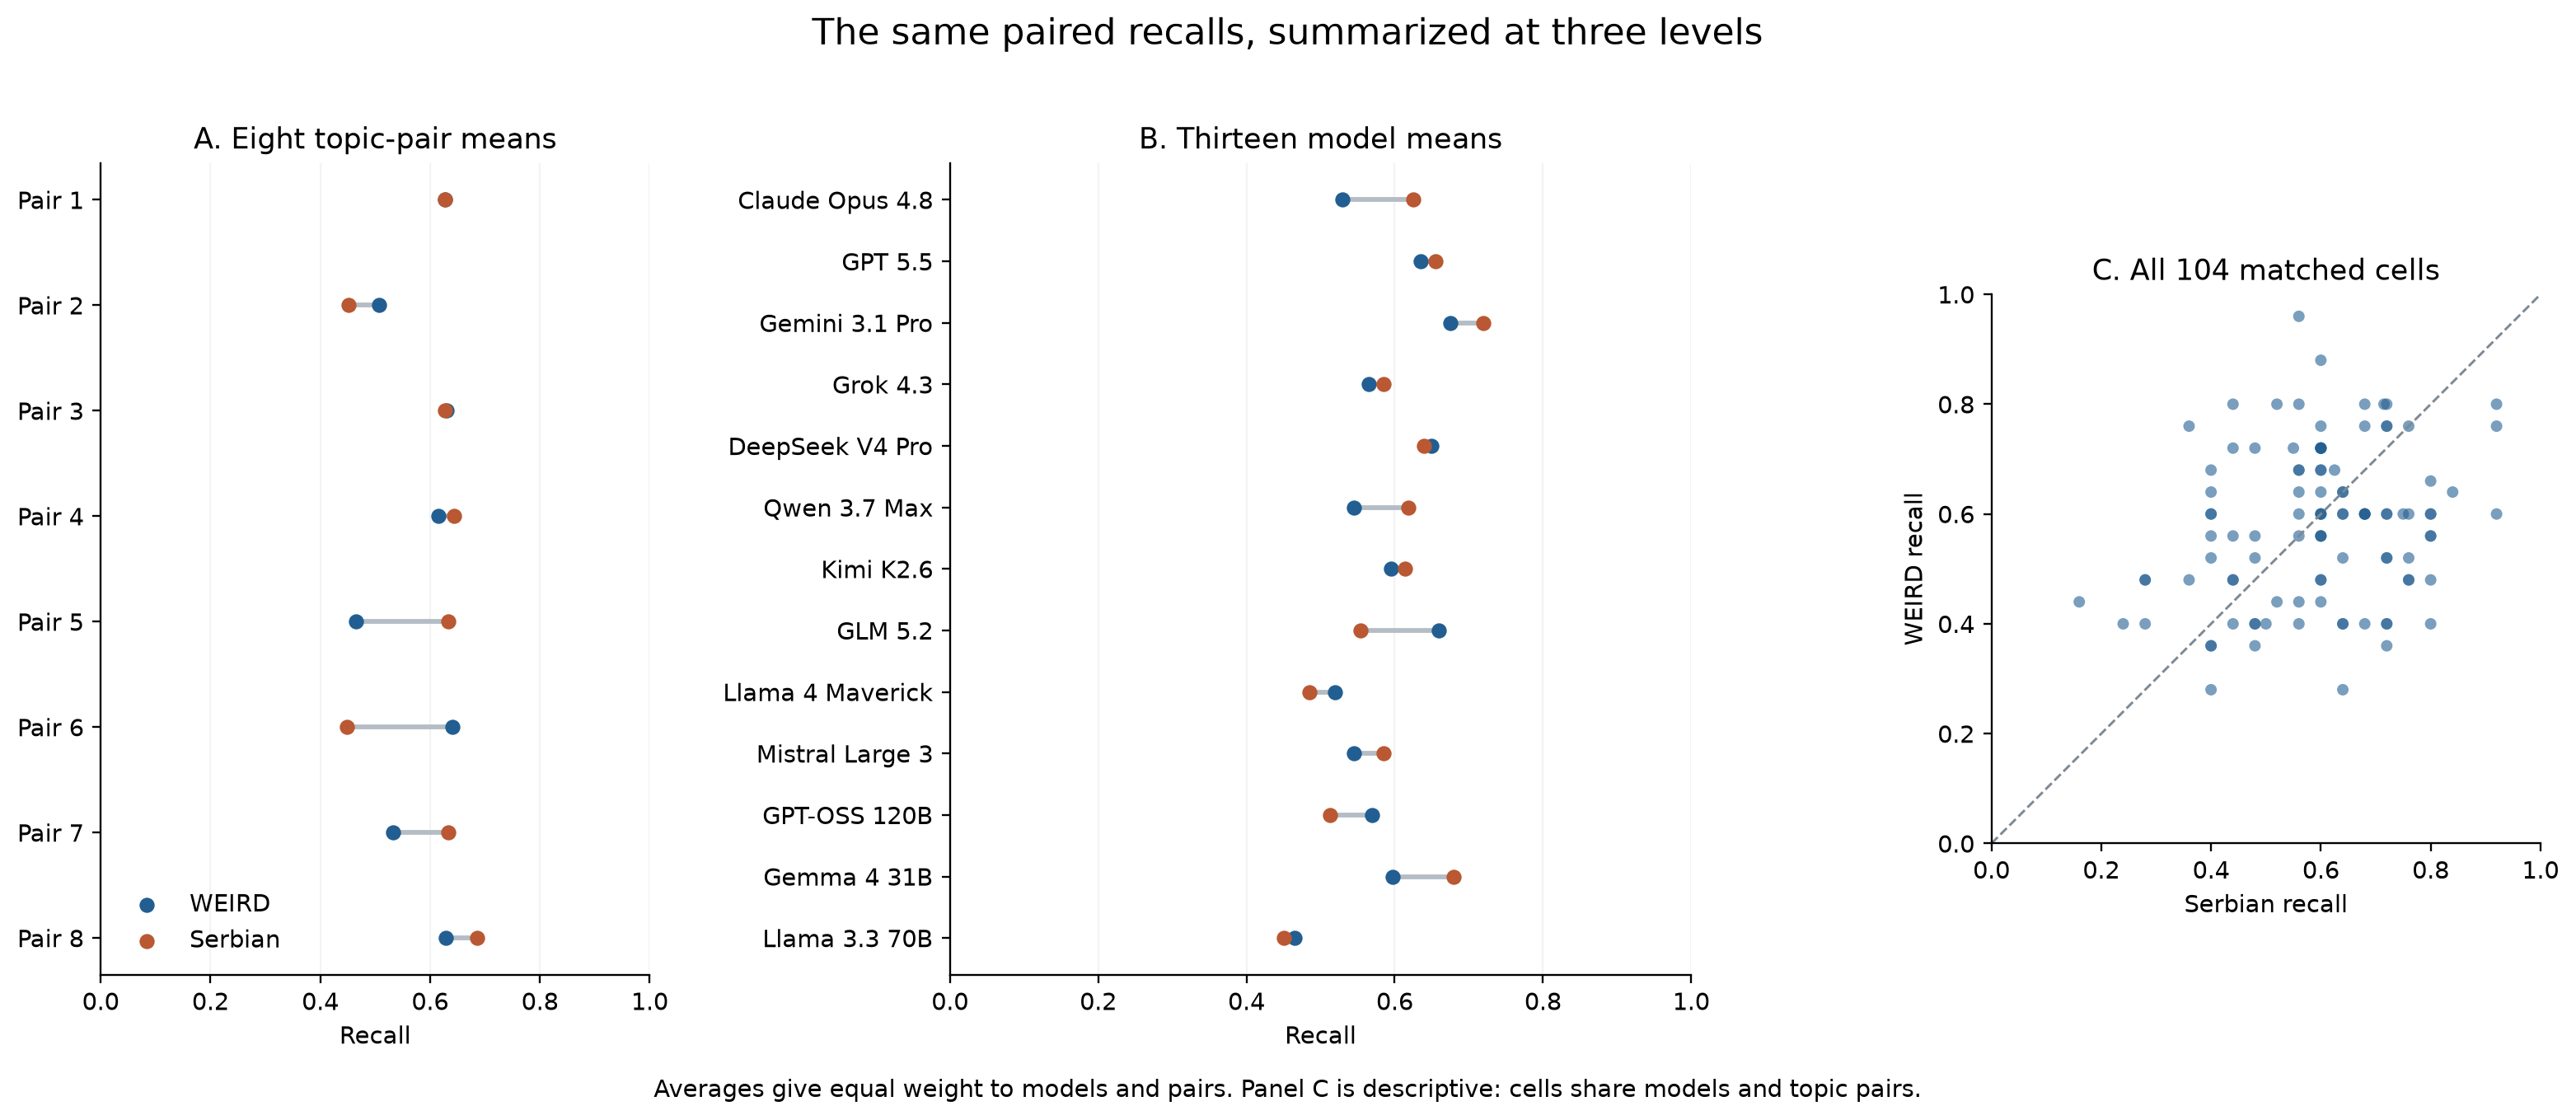
\includegraphics[width=\textwidth]{paired_recall.png}
\caption{Paired recall at three levels. Panel A averages the 13 generators
within each matched topic pair. Panel B averages the eight pairs within
each generator. Panel C plots all 104 model--pair comparisons, with the
dashed line indicating equal recall. Points above the line favour WEIRD
topics. Panel C is descriptive: its observations share generators and
matched topic pairs and are not independent replicates.}
\label{fig:paired-recall}
\end{figure}

\subsection{RQ2: Recall by model and access category}
\label{sec:rq2}
Table~\ref{tab:model-recall} reports perspective recall, with separate
columns for WEIRD and Serbian topics. Overall recall ranges from 0.458
for Llama 3.3 70B to 0.698 for Gemini 3.1 Pro. Even the highest-recall
model leaves approximately 30\% of the reference coverage unrecovered
on average.

\begin{table}[H]
\centering
\small
\caption{Perspective recall by access category, ordered by
overall recall within each category. Serbian topics constitute the non-WEIRD
arm. Overall intervals are the original 95\% bootstrap intervals over
16 topics; cultural-arm columns are means over eight topics. The
Frontier/API group includes Qwen 3.7 Max; larger and smaller open-weight
systems are shown separately. These group labels are not a capability ranking.}
\label{tab:model-recall}
\begin{tabular}{lccc}
\toprule
Model & Overall recall (95\% CI) & WEIRD & Serbian \\
\midrule
\multicolumn{4}{l}{\textit{Frontier/API systems (5)}}\\
Gemini 3.1 Pro & $0.698$ ($0.630$--$0.765$) & $0.675$ & $0.720$\\
GPT 5.5 & $0.645$ ($0.600$--$0.692$) & $0.635$ & $0.655$\\
Qwen 3.7 Max & $0.582$ ($0.524$--$0.639$) & $0.545$ & $0.618$\\
Claude Opus 4.8 & $0.578$ ($0.512$--$0.643$) & $0.530$ & $0.625$\\
Grok 4.3 & $0.575$ ($0.522$--$0.625$) & $0.565$ & $0.585$\\
\addlinespace
\multicolumn{4}{l}{\textit{Open-weight systems (6)}}\\
DeepSeek V4 Pro & $0.645$ ($0.560$--$0.730$) & $0.650$ & $0.640$\\
GLM 5.2 & $0.607$ ($0.542$--$0.667$) & $0.660$ & $0.554$\\
Kimi K2.6 & $0.604$ ($0.548$--$0.656$) & $0.595$ & $0.614$\\
Mistral Large 3 & $0.565$ ($0.485$--$0.640$) & $0.545$ & $0.585$\\
GPT-OSS 120B & $0.541$ ($0.468$--$0.612$) & $0.570$ & $0.513$\\
Llama 4 Maverick & $0.502$ ($0.432$--$0.580$) & $0.520$ & $0.485$\\
\addlinespace
\multicolumn{4}{l}{\textit{Small open-weight systems (2)}}\\
Gemma 4 31B & $0.638$ ($0.578$--$0.698$) & $0.598$ & $0.679$\\
Llama 3.3 70B & $0.458$ ($0.400$--$0.518$) & $0.465$ & $0.450$\\
\bottomrule
\end{tabular}
\end{table}

The mean recall of the selected models is 0.615 in the Frontier/API group,
0.578 in the larger open-weight group, and 0.548 in the smaller open-weight
group. Combining the eight open-weight models gives mean recall 0.570,
compared with 0.615 for the five API systems, an observed difference of
4.5 percentage points. The exact pair-blocked test gives $p=0.086$
before correction and $p=0.258$ after Holm correction across the four
RQ2 contrasts. None of those four comparisons meets the 0.05 threshold
after correction; the smallest adjusted value is $p=0.063$ for the API
versus smaller open-weight comparison. These exploratory results do not
establish equivalence or isolate the effects of size, openness, or capability.

Individual models also vary substantially within categories. Gemma 4 31B
has recall 0.638, close to the 0.645 reported for GPT 5.5 and DeepSeek
V4 Pro, whereas Llama 3.3 70B has recall 0.458. A category mean therefore
does not describe every model in that category. Overlapping individual
confidence intervals should not be interpreted as evidence of equivalence.

\subsection{RQ3: US and Chinese developer groups}
\label{sec:rq3}
The four selected models from Chinese developers have mean overall
recall 0.609, compared with 0.579 for the eight models from US developers
(Table~\ref{tab:origin-recall}). The US-minus-China difference is
$-0.030$ (95\% pair-bootstrap CI $[-0.048,-0.013]$). The exploratory
two-sided pair-blocked sign-flip test gives $p=0.023$, or $p=0.047$
after Holm correction across the two RQ3 outcomes.

\begin{table}[H]
\centering
\small
\caption{Recall by developer group. Models receive equal weight within
each group. Mistral is excluded from this US--China contrast. A positive
WEIRD--Serbian gap indicates higher recall on WEIRD topics.}
\label{tab:origin-recall}
\begin{tabular}{lccccc}
\toprule
Group & Models & Overall & WEIRD & Serbian & Gap\\
\midrule
US & 8 & $0.579$ & $0.570$ & $0.589$ & $-0.019$\\
China & 4 & $0.609$ & $0.613$ & $0.606$ & $+0.006$\\
\bottomrule
\end{tabular}
\end{table}

The groups' cultural gaps differ less conclusively. The mean
WEIRD-minus-Serbian gap is $-0.019$ in the US group and $+0.006$
in the Chinese group. Their difference is $-0.025$ (95\% pair-bootstrap
CI $[-0.082,0.025]$; raw and Holm-adjusted $p=0.453$). The observed
overall-recall difference therefore does not establish a corresponding
difference in the WEIRD--Serbian gap.

These results describe the selected systems. The Chinese group contains
one API and three larger open-weight models, whereas the US group contains
four API, two larger open-weight, and two smaller open-weight models.
The US group also includes multiple models from some developers. Developer country
is consequently entangled with model selection and category composition.
The comparison does not establish a general advantage of Chinese models
or a causal effect of developer location.

\subsection{Descriptive checks on judge consistency}
\label{sec:judge-checks}
Agreement statistics have similar values for WEIRD and Serbian topics
(Table~\ref{tab:judge-checks}). Fleiss' $\kappa$ is 0.761 for WEIRD
topics and 0.774 for Serbian topics. Gwet's AC1 and Krippendorff's
$\alpha$ show the same descriptive pattern. The judge-level no-match
rates are 32.9\% and 31.1\%, respectively.

\begin{table}[H]
\centering
\small
\caption{Descriptive inter-judge agreement. These statistics assess
consistency of matching decisions, not correctness or absence of shared bias.}
\label{tab:judge-checks}
\begin{tabular}{lccc}
\toprule
Scope & Fleiss' $\kappa$ & Gwet's AC1 & Krippendorff's $\alpha$\\
\midrule
All topics & $0.768$ & $0.783$ & $0.769$\\
WEIRD topics & $0.761$ & $0.777$ & $0.762$\\
Serbian topics & $0.774$ & $0.789$ & $0.775$\\
\bottomrule
\end{tabular}
\end{table}

Removing one judge at a time leaves the highest-recall model unchanged
and produces small changes in the pooled WEIRD-minus-Serbian gap,
which ranges from approximately $-0.020$ to $-0.008$ across removals.
These checks provide no obvious indication of substantially lower
agreement for Serbian topics or dependence of the pooled result on
one judge. They are descriptive checks, not formal demonstrations that
the panels have equal error rates. Several judges may agree on an
incorrect match, and shared cultural biases remain possible.

\section*{Conclusion: suggested updated passage}
Across eight matched WEIRD--Serbian topic pairs and 13 generators,
we did not detect the predicted WEIRD recall advantage. Coverage
nevertheless remained incomplete in both settings, and recall varied
across models and controversies. Exploratory comparisons described
variation among the selected model categories and higher overall recall
in the selected Chinese developer group, but did not establish a
US--China difference in the cultural recall gap. The category and
country comparisons are limited by the composition of the model sample.
The primary methodological implication remains that perspective
coverage should be measured directly using comparisons that account
for topic selection.

\clearpage
\section*{Supplementary metrics: retain outside the main recall table}
% Move the original precision/F1 table here rather than discarding its results.
Precision describes the share of generated outputs that match any
reference. In the single-judge example $(1,2,2,4,\text{no match})$,
precision is $4/5=0.80$, whereas recall is $3/5=0.60$. Duplicate matches
can contribute to precision without adding reference coverage.

For output $k$, let $b_{jk}=1$ when judge $j$ selects any reference
and $b_{jk}=0$ for a valid no-match decision. The output's precision
credit and the topic precision are
\[
q_k=\frac{1}{|J_k|}\sum_{j\in J_k}b_{jk},
\qquad P_{mt}=\frac15\sum_{k=1}^{5}q_k.
\]
Model precision averages the 16 topic precisions. Model F1 is calculated
from model-level mean precision and mean recall,
\[
F1_m=\frac{2\overline P_m\overline R_m}{\overline P_m+\overline R_m},
\]
rather than by averaging judge-level or topic-level F1 values. These
metrics are supplementary because an output outside the five-reference
set may still express a legitimate position. Thus, an unmatched output
does not by itself establish invalid content, and the main omission
analysis uses recall.

\end{document}
